%%%%%%%%%%%%%%%%%%%%%%%%%%%%%%%%%%%%%%%%%%%%%%%%%%%%%%%%%%%%%%%%%%%%%%%%%%
% Copyright (c) 2011, ETH Zurich.
% All rights reserved.
%
% This file is distributed under the terms in the attached LICENSE file.
% If you do not find this file, copies can be found by writing to:
% ETH Zurich D-INFK, Haldeneggsteig 4, CH-8092 Zurich. Attn: Systems Group.
%%%%%%%%%%%%%%%%%%%%%%%%%%%%%%%%%%%%%%%%%%%%%%%%%%%%%%%%%%%%%%%%%%%%%%%%%%

\documentclass[a4paper,11pt,twoside]{report}
\usepackage{bftn}
\usepackage{calc}
\usepackage{verbatim}
\usepackage{xspace}
\usepackage{pifont}
\usepackage{textcomp}
\usepackage{amsmath}

% Include the listings-package
\usepackage{listings}
\lstset{
	basicstyle=\footnotesize\ttfamily,
	framexbottommargin=4pt,
	frame=single,
	basicstyle=\footnotesize, 
	captionpos=b
}

\usepackage{float}
\newfloat{code}{H}{myc}

\usepackage{bytefield}

\newcommand{\HRule}{\rule{\linewidth}{0.5mm}}

\title{Tracing and Visualisation}
\author{Barrelfish project}
% \date{\today}		% Uncomment (if needed) - date is automatic
\tnnumber{8}
\tnkey{Tracing}

\begin{document}
\maketitle			% Uncomment for final draft

\begin{versionhistory}
\vhEntry{1.0}{28.02.2013}{Alexander Grest, David Stolz}{Initial version}
\end{versionhistory}

% \intro{Abstract}		% Insert abstract here
% \intro{Acknowledgements}	% Uncomment (if needed) for acknowledgements
% \tableofcontents		% Uncomment (if needed) for final draft
% \listoffigures		% Uncomment (if needed) for final draft
% \listoftables			% Uncomment (if needed) for final draft


\chapter{Overview}

The tracing framework in Barrelfish consists of three major components:

\begin{itemize}
	\item The tracing library.
	\item Bfscope (a Barrelfish program).
	\item Aquarium 2.
\end{itemize}

The tracing library can be used to instrument code in order to trace events.
The events are stored core local and can later be flushed, either to console
or -- with the help of Bfscope -- to a remote machine. On the remote machine
you can analyze the trace data using Aquarium 2. Aquarium 2 can be customized with scripts,
making it easy to integrate specific needs into the existing analysis framework.
In addition it supports various export functionalities that allow you to analyze
trace data with external tools in an easy fashion.

\chapter{Design and Implementation of the Tracing Framework in Barrelfish}

\section{Overview\label{sec:trace-overview}}

The tracing framework inside of Barrelfish existed already before this project
has been started. In order to break as little as possible in existing code to
work with the tracing system (e.g.~tools that have been developed analyzing
trace logs) we decided to change as little as possible on the interface of the
tracing framework. In the end the structure of the trace logs that are generated
did not change, but only some mappings between constants in code and their
interpretation. 

In this section we want to look at the part of the tracing framework that is
implemented in Barrelfish, i.e.~the actual functionality that developers use in
order to create trace logs. One part of the tracing framework allows developers
to trace events at any point in the code, where the data that is actually stored
is defined in the Section \ref{sec:trace-event}. The second part is responsible
for delivering the generated trace logs to Aquarium. To achieve the second goal
we changed the existing Barrelfish application Bfscope in such a way, that it
integrates with the new version of the tracing framework. Bfscope is described
in Section \ref{sec:bfscope}.

The typical lifecycle of using the tracing framework in Barrelfish looks like
this:

\begin{description}
	\item[0.a (Optional)] Prepare the tracing framework.
	\item[0.b (Optional)] Specify which Subsystems should be logged.
	\item[1.] Define the type of event that will trigger the start of tracing.
	\item[2.] \emph{Execute your code, that will log the events.}
	\item[3.] Flush the logged events, e.g.~on the console.
\end{description}

To get more information about the optional steps, see Sections
\ref{sec:preparing} and \ref{sec:enabling-disabling}. The first mandatory step
is to define the type of the event that will start the logging process. Having a
mechanism for starting and stopping the actual tracing may seem like a benefit,
but not like a necessity at first -- but our experiments have shown that even
with rather small instrumentation of code (i.e.~number of events that actually
generate an entry in the trace log), having the tracing framework log events all
the time is no option. Thus having the possibility to start and stop the tracing
framework is essential. Having the flexibility of specifying a type of trace
event that will trigger the start and stop of the logging is an additional
benefit compared to having simple ``start'' and ``stop'' commands, as it allows
developers to easily vary the portion of code they want to trace, without
changing the placement of a ``start'' and ``stop'' command all the time.

While the second mandatory step is pretty self-explanatory, the third step is
more interesting again: The old version of the tracing system allowed only for
dumping the stored trace into a provided buffer. This functionality has now been
improved in such a way that we offer developers a method to flush the current
trace log, and the flush functionality automatically detects the best way to
flush. Currently there are two possible destinations onto which can be flushed:
The console and the network. The tracing framework detects automatically if
Bfscope is running and someone is connected to it -- if so, it flushes over the
network -- else it will flush to the console. The flushing functionality could
also be extended, a possible idea would be to store the trace log in a file. In
Figure \ref{fig:flush} you can see a sequence diagram illustrating the process
of invoking the new flushing functionality.

\begin{figure}[t]
	\begin{center}
		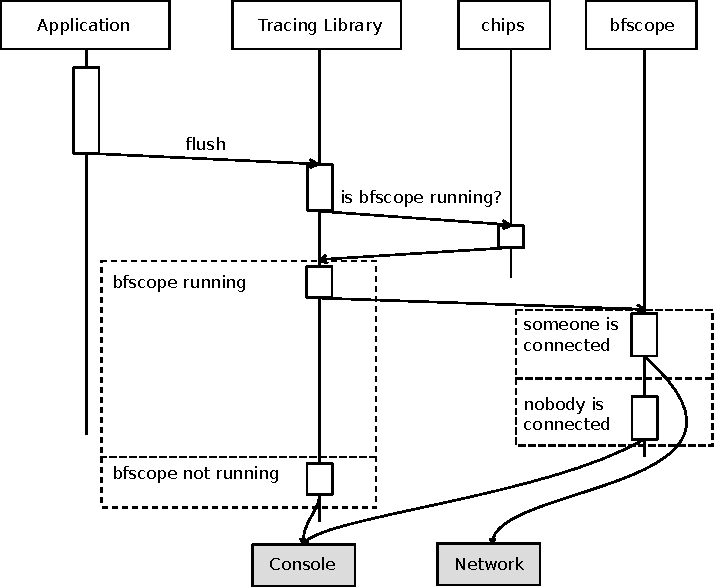
\includegraphics{images/flush.pdf}
	\end{center}
	\caption{A sequence diagram illustrating the flow of events when using the
	flush functionality. ``Application'' is the application that is using the
tracing framework, and chips is the Barrelfish nameserver. The grey boxes
indicate the destination onto which is flushed.}
	\label{fig:flush}
\end{figure}


\section{Definition of a Trace Event\label{sec:trace-event}}

Let us now define the structure of events that can be traced. Each event
belongs to a Subsystem and an Event, and has an optional payload called Argument
that can hold 32 bits of arbitrary information. Both the Subsystem and the Event
are 16 bit identifiers, allowing us to have up to 65535 Subsystems and for each
Subsystem 65535 Events. Note that the Events are relative to the Subsystems,
i.e.~a Subsystem called \emph{kernel} might have the Event \emph{Context Switch}
with the identifier 0, but the same Event identifier 0 has an entirely different
meaning in every other Subsystem.

Having all these different Subsystem and Event identifier available, we think
that the tracing framework will have sufficient space to deal with future change
in Barrelfish\footnote{Currently there exist 16 different Subsystems.}.

In addition to the Subsystem, Event and Argument information, the tracing
framework adds a timestamp to each event that gets logged (the timestamp is
measured in CPU cycles) and remembers the core on which the event was logged. The core is
only implicitly stored, as we have a separate tracing buffer on each core,
allowing us to identify the core for an event at a later stage automatically,
without storing it for each event.

As timestamps are stored as a 64 bit number, we need a total of 128 bits
(respectively 16 bytes) per event that has been logged. The data structure
layout of a single event can be seen in Figure \ref{fig:trace-event}.

\begin{figure}[t]
	\begin{center}

		\begin{bytefield}[bitwidth=0.2cm]{64}
			\bitheader{0,16,32,48,63} \\
			\bitbox{64}{Timestamp} \\
			\bitbox{16}{Subsystem}
			\bitbox{16}{Event}
			\bitbox{32}{Argument}

	\end{bytefield}

	\end{center}
	\caption{Representation of a single trace event in memory in Barrelfish.}
	\label{fig:trace-event}
\end{figure}

\section{Pleco: A new Domain Specific Language}

\subsection{Overview}

As trace events are identified by the type of their Subsystem and Event (which
is a two tier hierarchical structure), the best way to specify those Subsystems
and Events is using a domain specific language. For this purpose we designed a
new domain specific language called \emph{pleco}, that resembles the domain
specific language for error codes in Barrelfish (called fugu) a lot -- due to
the fact that it solves a very similar task.

Pleco allows programmer to easily add new Subsystems to the tracing framework
and to extend existing Subsystems with new Events. Note that the Argument
parameter of the trace events is not specified in Pleco, as this parameter is
intended to be a payload, and not to be a means to distinguish different trace
events. A small sample pleco file can be seen in Listing
\ref{lst:pleco-file}. In this file we define two Subsystems: \texttt{kernel} and
\texttt{memserv}. Note that the keyword \emph{subsystem} is used to define a new
Subsystem. The Events for a Subsystem are defined in the block following its
name. Events have both a name and a verbose description, following the keyword
\emph{event}. The textual description is \emph{not used} in the tracing framework
inside of Barrelfish, but Aquarium will use the textual description to display
it when analyzing generated traces. Note that the textual description is not a
strict requirement; if the empty string is provided, during the interpretation
of the pleco file, the name of the event will be substituted for the textual
description.

\begin{code}
\begin{lstlisting}[frame=single, caption={A small example pleco file with two
	Subsystems.}, label={lst:pleco-file}]
subsystem kernel {

	event CSWITCH               "Context Switch",
	event BZERO                 "Buffer zeroing",
	event TIMER                 "", 
	event TIMER_SYNC            "", 

};

subsystem memserv {

	event ALLOC	             "", 
};
\end{lstlisting}
\end{code}

\subsection{Interpreting Pleco Files}

Parsing and interpreting of pleco files is part of the Barrelfish build process,
meaning that the according tools are written in Haskell and are integrated into
the Hake build process.  An overview of how pleco files are integrated into the
Barrelfish toolchain can be seen in Figure \ref{fig:pleco-process}. Note that
the header file that is created during the build process is directly used in the
very same build process, i.e.~it is just an intermediate file.

\begin{figure}[t]
	\begin{center}
		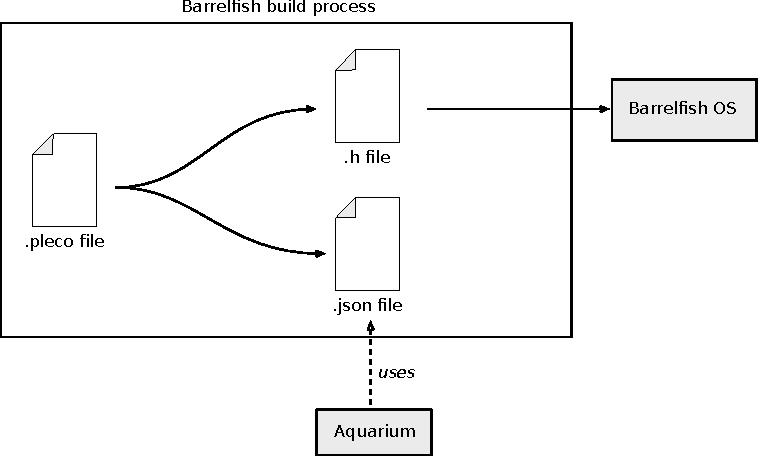
\includegraphics{images/pleco-process.pdf}
	\end{center}
	\caption{Pleco files get translated into both a C header file and a JSON
	file. This translation is taking place during the regular build process of
Barrelfish.}
	\label{fig:pleco-process}
\end{figure}

\subsection{The Generated Header File}

For the pleco file of Listing \ref{lst:pleco-file}, the header file shown in
Listing \ref{lst:headerfile} has been generated during the build process. In
Barrelfish source code, this file can be included with the statement:

\begin{description}
	\item[$\#$include] <trace\_definitions/trace\_defs.h>
\end{description}

Note that the macro that are created for events also contain the subsystem name,
so that there will not be any name collisions when two different subsystem
define an Event with the same name.

The generated numbers are not randomized. The reason for this is not that people
can avoid using macros, but rather for a new feature that has been introduced
into the tracing framework to work: enabling and disabling of Subsystems that
are logged. See Section \ref{sec:enabling-disabling} for detailed information.

\begin{code}
\begin{lstlisting}[frame=single, caption={A header file that has been generated
	based on the pleco file shown in Listing \ref{lst:pleco-file}.}, label={lst:headerfile}]
#ifndef TRACE_DEFS_BARRELFISH__                                                          
#define TRACE_DEFS_BARRELFISH__

#define TRACE_SUBSYS_KERNEL 0
#define TRACE_EVENT_KERNEL_CSWITCH  0
#define TRACE_EVENT_KERNEL_BZERO    1
#define TRACE_EVENT_KERNEL_TIMER    2
#define TRACE_EVENT_KERNEL_TIMER_SYNC   3

#define TRACE_SUBSYS_MEMSERV    1
#define TRACE_EVENT_MEMSERV_ALLOC   0


#define TRACE_NUM_SUBSYSTEMS    2

#endif // TRACE_DEFS_BARRELFISH__ 

\end{lstlisting}
\end{code}

\subsection{The Generated JSON File}

As the pleco file shown in Listing  \ref{lst:pleco-file} does not only get
translated into a header file, but also into a JSON file, we want to have a look
at this file now. The JSON file that has been generated for said pleco file can
be seen in Listing \ref{lst:jsonfile}.

\begin{code}
\begin{lstlisting}[frame=single, caption={A JSON file that has been generated
	based on the pleco file shown in Listing \ref{lst:pleco-file}. This file can
be used by Aquarium to decode log traces.}, label={lst:jsonfile}]
{                                                                                        
0 : { 
    "name" : "kernel",
    "events" : { 
        0 : "Context Switch",
        1 : "Buffer zeroing",
        2 : "TIMER",
        3 : "TIMER_SYNC"
    }   
},
1 : { 
    "name" : "memserv",
    "events" : { 
        0 : "ALLOC"
    }   
}
}
\end{lstlisting}
\end{code}

As you can see, the textual description in the pleco file was used where
provided, and where it wasn't, the name of the Event has been used as a
substitution. The generated numbers are the same as the ones in the header file.
This is no coincidence, as the usage of this JSON file is exactly to decode the
numbers from the trace logs into human readable events again.

For the purpose of decoding the events, the old version of Aquarium had the
mapping from numbers to human readable events directly hard coded into the
source code. This new way of defining Subsystems and Events in pleco files
allows programmers to omit duplicate work (and having to check that both programs
are always consistent), and provides them with an automated way of having a
consistent tracing framework and analysis tool.

\section{Feature Overview}
\subsection{Preparing the Tracing Framework\label{sec:preparing}}

The tracing framework does not strictly need any extra preparation, nevertheless
depending on the environment, a preparation might be necessary. For this reason
we added the functionality to prepare the tracing framework. Currently the
preparation process estimates the offset between the CPU cycle counters on the
different cores. This functionality is not needed on machines that have
synchronized cycle counters, but in the future it might be possible to run a
single instance of Barrelfish on multiple machines, and in this case the
different cycle counters will not be synchronized anymore.

The cycle counter offsets are all measured relative to core $0$. To measure the
offset between a core $i$ and core $0$, we execute the Network Time Protocol
clock synchronization algorithm 
between the two cores. Figure \ref{fig:ntp} illustrates the steps of the clock
synchronization between two cores. Four time measurements are performed and the
estimated offset $\theta$ between the two cores is calculated as follows:

\begin{equation}
	\theta =  \frac{(t_1-t_0)+(t_2-t_3)}{2}
\end{equation}

\begin{figure}[t]
	\begin{center}
		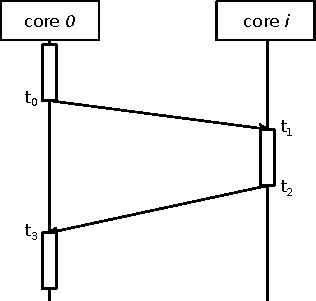
\includegraphics{images/ntp.pdf}
	\end{center}
	\caption{NTP clock synchronization. Four time measurements $t_0$ to $t_3$
	are performed. }
	\label{fig:ntp}
\end{figure}

The tracing framework performs measurements between every core $i$ ($i > 0$) and
core $0$ sequentially, so that the measurements are as precise as possible. The
messages needed to perform those measurements are sent using the monitor,
meaning that the tracing framework does not need to setup any new channel.

\subsection{Enabling and Disabling of Events\label{sec:enabling-disabling}}

With the new version of Aquarium it is possible to filter out events in the
analysis for a given trace log. But it showed that this functionality is not
sufficient, as there are use cases where applications log so many events, that
filtering must already be performed on the fly, i.e.~already during the tracing
process itself. An application where this is currently necessary in Barrelfish
is the tracing of the network stack. The current way of achieving this filtering
is introducing preprocessor statements at different locations in the code.
Having the new domain specific language available, we implemented a mechanism to
enable and disable Subsystems directly at runtime, using the Subsystem
identifier generated from the pleco file.

It is now possible to change which Subsystems are logged directly at runtime,
removing the need of recompiling the entire tracing framework just because the
type of events that a developer is interested changed. With the hierarchical
structure of Subsystems and Events it was possible to implement this enabling
facility in a lightweight manner, as the number of Subsystems is quite small.


\subsection{Automatic Flushing}

The flush procedure described in Section \ref{sec:trace-overview} can be
triggered by manually calling the according trace framework function. In
addition to the manually triggered flushing, we added a new functionality,
namely the one that the trace buffer is flushed automatically. This
functionality is implemented with in Bfscope, as we think the main use-case for
automatic flushing is when the generated logs are automatically forwarded to a
remote machine\footnote{Having the console cluttered with events from the
tracing framework can render the application unusable rather quickly.}. When a
developer decides to enable the automatic flushing and Bfscope is running,
Bfscope will automatically flush the content of the trace buffers periodically.
This feature removes the need of having to call the flush procedure manually,
but it developers should note that if timing is critical for your application,
the automatic flushing functionality can lead to issues. The issues that can
arise come from the fact that it is possible that Bfscope flushes in the middle
of your application executing its code -- this does not lead to a problem of
correctness, but it can heavily skew the flow of events in the Barrelfish as a
whole.

\section{Bfscope\label{sec:bfscope}}

Bfscope is a Barrelfish program that enhances the functionality of the tracing
framework by the possibility to directly flush trace logs over the network. Note
that the tracing in the Barrelfish code itself runs independently of Bfscope --
and it even notices when Bfscope is running and changes its behavior
accordingly. Bfscope allows developers to connect from a remote machine to the
Barrelfish OS, using a TCP connection and to get the trace logs directly onto
the remote machine. Note that when a remote machine is connected, regular flush
commands in Barrelfish will automatically be redirected onto the network, and
you will not see the trace logs on the console any longer.

As the remote machine is merely a utility that wants to get the trace log data,
there are no messages exchanged as part of a protocol -- Bfscope simply sends
the trace log data onto the TCP connection, once the flush command is issued (or
periodically if automatic flushing is enabled). This has, beneath being a simple
protocol, the additional benefit that it is no longer necessary to run Aquarium
in order to be able to get the trace log onto a remote machine, but you rather
can use any tool that allows you to open a TCP connection, such as netcat. Using
such a tool will allow you to get the trace log data on a different machine,
where you can either later analyze it with Aquarium, or with custom scripts.

Nevertheless the main intention is to directly connect to Bfscope using
Aquarium, which can interpret and visualize the trace log data directly on the
fly.

% ----------------
\chapter{Design and Implementation of the Analysis Tool Aquarium\label{sec:aquarium}}

\section{Design of Aquarium}

\subsection{Goals}

When we designed Aquarium we had several goals in mind, namely the following
ones:

\begin{enumerate}
	\item Support for live tracing.
	\item Support for different ways of input (e.g.~reading from file or
		receiving data over the network).
	\item Being able to handle large trace log data.
	\item Being extensible and easily customizable.
	\item Aquarium must run on different operating systems.
\end{enumerate}

We decided to tackle the first three goals with the design of the architecture
of Aquarium, which we will discuss in Section \ref{sec:aquarium-architecture}.
The fourth goal also did influence the architecture on one hand, but also
led to the idea of making Aquarium scriptable, i.e.~to create an interface that
allows developers to add their own scripts to Aquarium. Since those scripts do
not work on the raw trace log data, but rather on already from Aquarium
interpreted data, it offers developers on one hand a more powerful means to
write scripts in a very easy way, and on the other hand the scripts are directly
integrated into the visualization of Aquarium, alleviating the need to write
visualization code for custom developer scripts. In Section \ref{sec:scripts} we
will discuss the different ways how Aquarium can be extended with scripts.

The fifth goal, i.e.~the goal that people should be able to run Aquarium on
different Operating Systems, such as Linux and Windows, arose from a shortcoming
in the old version of Aquarium -- namely that it was written in C\# and only
runs on Windows. To tackle this requirement we decided to implement our version
of Aquarium in Java, so that cross platform portability will certainly not
become an issue.

\subsection{Architecture\label{sec:aquarium-architecture}}

When you analyze trace log data with Aquarium, the main object is a
TracingSession object. Each trace log data is at runtime represented by exactly
one TracingSession object. Figure \ref{fig:classdiag-input} shows the most
important classes that are dealing with getting from trace log data to the
according TracingSession. A TracingSession is associated with a single event
provider, currently there are two different input ways implemented:

\begin{itemize}
	\item Reading trace log data from a file, using a LogfileReader.
	\item Reading trace log data directly from a Barrelfish machine, using a
		NetworkReader.
\end{itemize}

The actual interpretation of the trace log data is done using an EventParser;
EventParser objects are independent of the type of data source. Note that the
EventConfigurtion is the responsible for interpreting the JSON file that has
been generated during the build process of Barrelfish, based on the pleco file.

The trace log data gets interpreted to Events and Activities, that are stored in
the TracingSession object. Note that the flow of data is push based, i.e.~it is
the data source that actively creates new Events as soon as more data is
available, and pushes the Events to the TracingSession. Having an active data
source allows us to treat different types of data sources uniformly.

While Events are quite self explanatory, i.e.~they are the Aquarium
representation of the actual events in the trace log data, Activities are a new
concept that we introduced in Aquarium. An Activity is a sequence of Events,
that are grouped into a single activity. Activities are a typical constructs
that are needed when analyzing trace log data; an example for that is when
analyzing the network stack, the fact that memory has been allocated (a single
event) might not be very interesting, but the duration of the entire
construction of the packet (an Activity) is what is actually very interesting.
Thinking about Activities, it becomes immediately clear that the different types
of Activities must be flexibly definable. We achieved this by allowing
developers to create their own scripts that decode Activities. 

\begin{figure}[htb]
	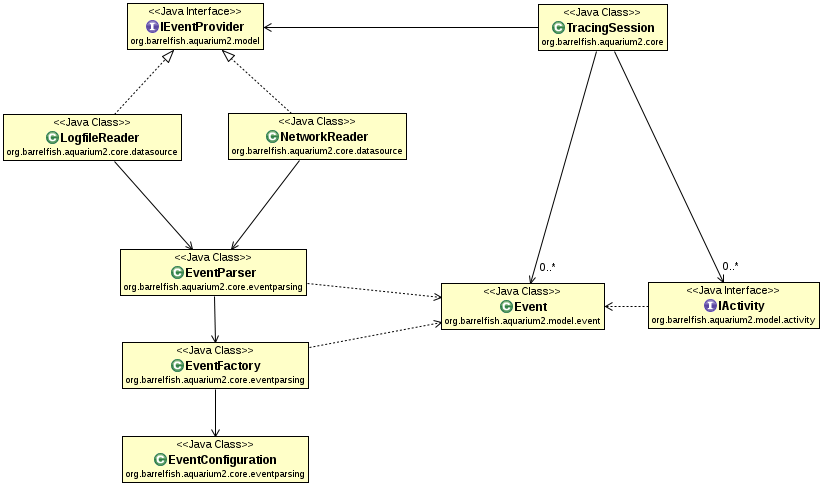
\includegraphics[width=1\textwidth]{images/classdiag-input.png}
	\caption{UML class diagram showing the main classes that are concerned with
		dealing with input.}
	\label{fig:classdiag-input}
\end{figure}

Let us now look at how events are processed once the TracingSession retrieves a new Event.
A class diagram illustrating the handling of Events and Activities can be seen
in Figure \ref{fig:classdiag-output}. A TracingSession stores both a list with
the Events that have been extracted from the trace log data, as a list with all
the activities that have been created based on those events. Once an Event is
received by the TracingSession, it notifies all registered EventHandlers to
handle the new Event. Such EventHandlers can either be UI elements, such as an
EventListUpdateHandler (an object being responsible to present a list of all
interpreted Events in the UI), or an ActivityDecoder. ActivityDecoders are
objects that create Activities, and one possibility for that is, as already
mentioned, to have external scripts which decode Activities. If an
ActivityDecoder creates a new Activity, this Activity will be added to the
TracingSession and all registered ActivityHandlers will receive it. As you can
see, the only module that is currently both receiving Events and Activities is
the GraphViewUpdateHandler, an object that is responsible for visualizing the
trace log data graphically.

When developing Aquarium, we initially planned to add a statistics module as
well. Due to a lack of time, we had to omit it in the end. Nevertheless from the
design it can be seen, that such a module could easily be added to Aquarium: It
would simply have to be an EventHandler and an ActivityHandler. Note that the
design with having the TracingSession at the core, we achieved that all handler
classes are always in a consistent state. For example if an activity is seen by
one handler, it is always also seen by all other handlers. This becomes
especially handy when considering the filtering functionality of Aquarium. In
Aquarium we added the functionality to filter out Events based on various
different criteria, ranging from the core on which the Event happened, over the
Subsystem type up to custom scripts that developers can write to create their
own filter. When a filter is applied, it is always applied on the
TracingSession, and not on e.g.~a UI element. With this globally applied
filtering mechanism a new Handler that is created to extend Aquarium would
immediately benefit from the filtering functionality, without having to take
care of it at all.

\begin{figure}[htb]
	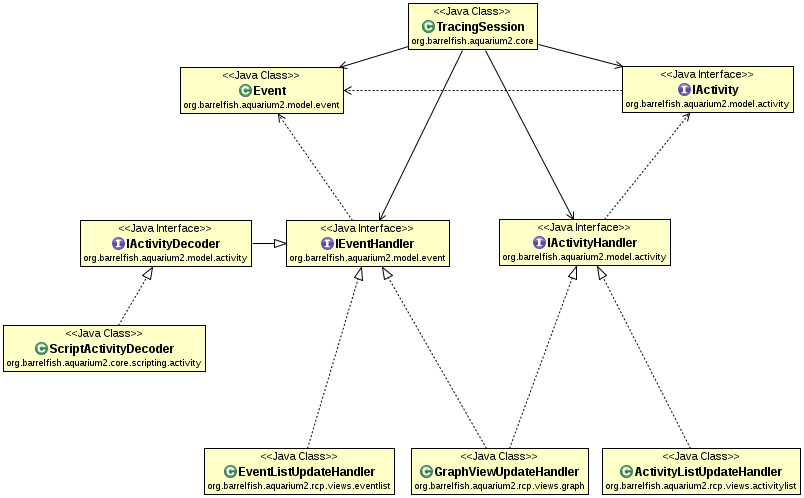
\includegraphics[width=1\textwidth]{images/classdiag-output.png}
	\caption{UML class diagram showing the main classes that are concerned with
	handling events and activities.}
	\label{fig:classdiag-output}
\end{figure}

\section{Extending Aquarium with Scripts\label{sec:scripts}}

As mentioned in Section \ref{sec:aquarium-architecture}, it is possible to
extend the functionality of Aquarium by adding custom scripts. The scripts are
interpreted using the Java Scripting API, and currently JavaScript is the
language for which support in Aquarium has been implemented. Based on the Java
Scripting API support for other languages could be added.

\subsection{Script Filters}

Script filters are custom scripts that can be written by developers to filter
out events in which they are not interested. Aquarium itself already provides
the possibility to filter out events based on the following criteria:

\begin{itemize}
	\item Filter out entire cores (e.g.~filter out core 1).
	\item Filter out entire Subsystems (e.g.~filter out the \emph{kernel}
		Subsystem).
	\item Filter out Events from a Subsystem (e.g.~filter out \emph{ALLOC}
		Events from the Subsystem \emph{memserv}).
	\item Filter out trace events based on their application (e.g.~filter out
		all events that the application \emph{monitor} logged).
\end{itemize}

If a user is not satisfied with these possibilities to filter out events,
Aquarium can be extended with script filters. An example for a script filter
would be to filter out all events, except those that are an \emph{ALLOC} Event
initiated by the monitor. Such scripts allow users to quickly spot specific
events, even when they are analyzing large trace logs.

\subsection{Script Activities}

Another possibility to extend Aquarium with the help of scripts is to write
custom activity scripts. Such a script works in the following way: It receives
all events that exist in the trace log, in the order they exist in the trace log
itself, and based on these events it can create activities, and deliver them to
Aquarium. In Figure \ref{fig:classdiag-output} we can see that such a Script is
wrapped in a ScriptActivityDecoder inside of Aquarium, which is -- as just
described -- an EventHandler.

An example for an activity script could be to create an activity for  all the
\emph{MUTEX\_LOCK} and \emph{MUTEX\_UNLOCK} pairs -- in order to analyze the
locking behaviour. For each activity, certain parameters such as the duration of
each activity, is automatically calculated by Aquarium.

\section{Working with Aquarium}

In this section we briefly want to look at how some of the already described
functionality looks in Aquarium with the help of some examples. Figure
\ref{fig:aquarium} shows a screenshot displaying a single trace log data file opened in
Aquarium. The largest part of the GUI is used by the so called \emph{GraphView},
presenting the information contained in the log in a two dimensional manner.
From left to right we see the timestamps (measured in clock cycles), and on the
vertical axis we see the different cores.

For each core we show the actual events that have been traced, indicated using
black circles on the bar of the core. The color of the bar shows which
application was running on the core on that time, where the colors are shown as
well in the left menu labeled \emph{Filter}. In addition to the per core events,
arrows are drawn where messages have been sent between the cores, indicating
the send and receive event. As the messages have the potential to clutter up the
GUI quite a bit, the arrows can be hidden easily using the envelope button on
the right top corner.

Below the GraphView we see a list representation of the event data. With the
help of the \emph{sync} button (shown on the right top corner of the list), the
GraphView and the list can be linked, meaning that if you select an event in
either of the two, the other view scrolls to that event. Using this
functionality coarse navigation can be done using the GraphView, to then allow
for detailed analysis by quickly looking at the list.

On the left part of the GUI we see the Filter menu. It allows to filter out
events based on the different criteria, as already described. Scripts can be
added using the Scripts tab, and afterwards they will directly appear in the
Filter menu as well.

\begin{figure}[htb]
	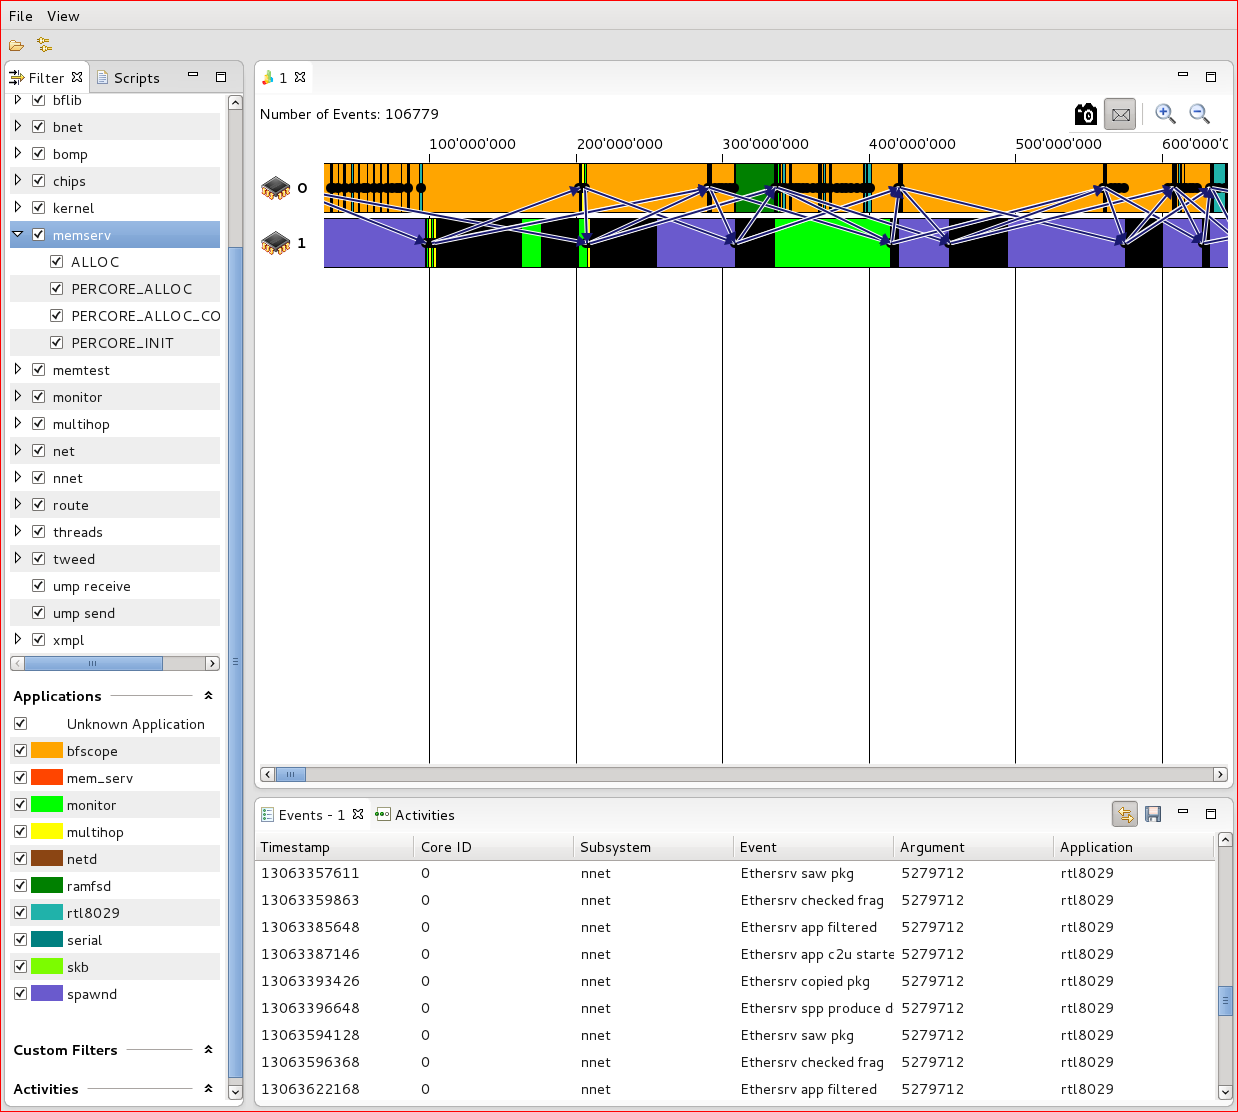
\includegraphics[width=1\textwidth]{images/aquarium.png}
	\caption{Screenshot of Aquarium displaying one trace log file.}
	\label{fig:aquarium}
\end{figure}

As we can see in the screenshot shown in Figure \ref{fig:aquarium-activities},
for all the objects in the GraphView exist tooltips, when you hover over the
according object with the mouse cursor. On this screenshot you can see that two
custom script activities have been added, and they have already been evaluated.
The created activities are integrated into the GraphView (on a per core basis)
as well as in the Activity tab next to the Events list on the bottom of a
Aquarium. All created activities can also be seen in a list fashion there.

\begin{figure}[htb]
	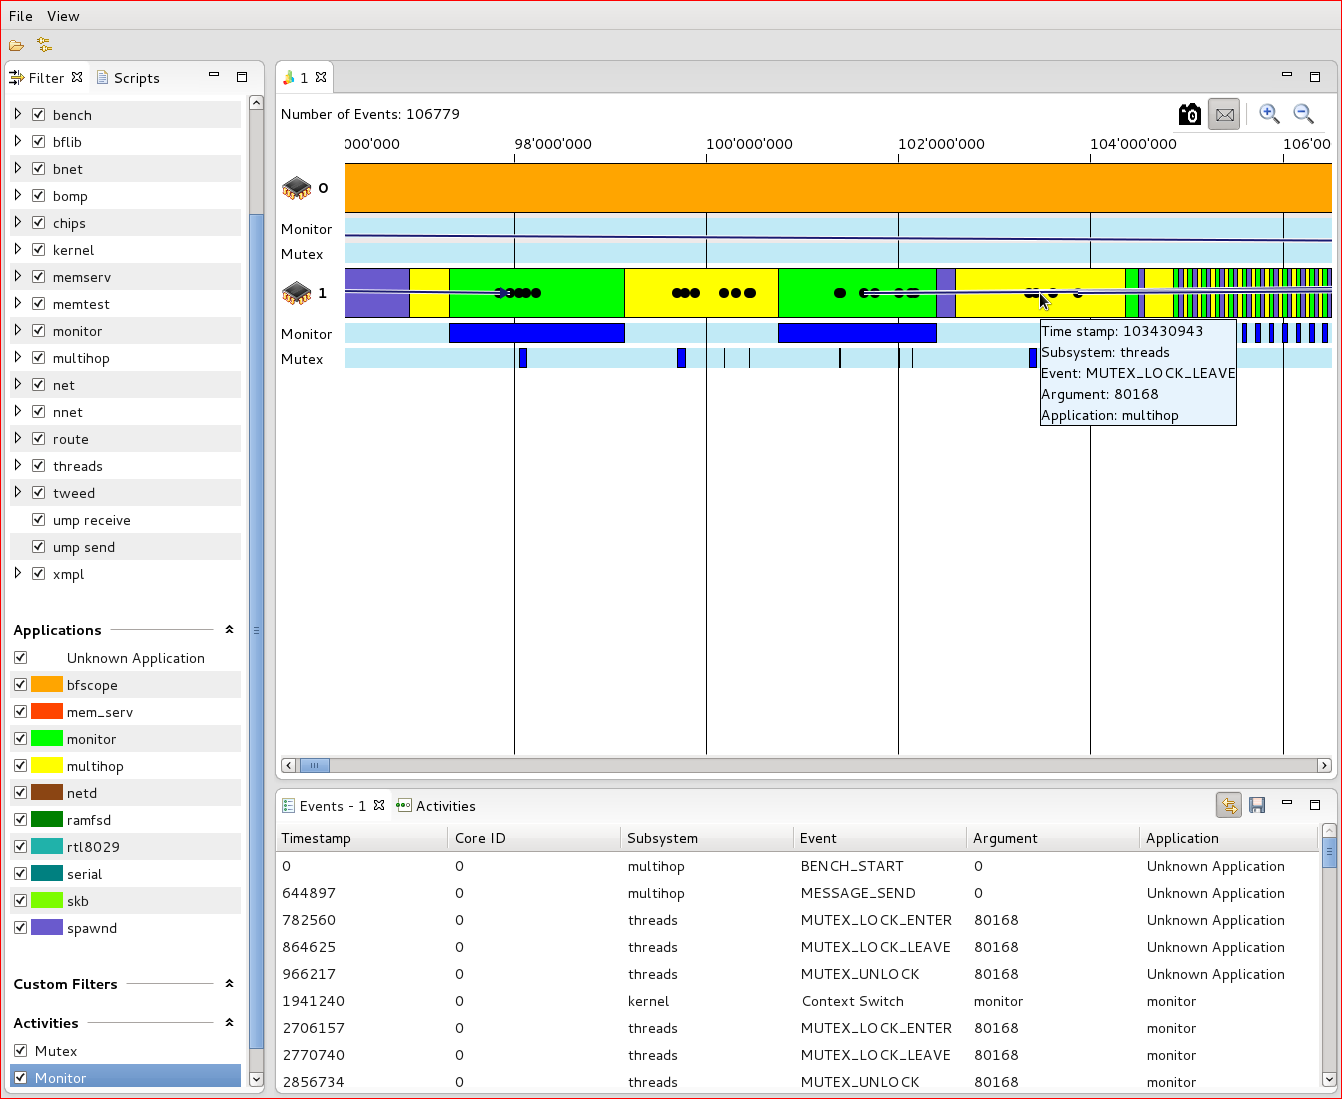
\includegraphics[width=1\textwidth]{images/aquarium-activities.png}
	\caption{Screenshot of Aquarium displaying two script activities, one for
	mutex activities and one for the monitor application.}
	\label{fig:aquarium-activities}
\end{figure}

In Figure \ref{fig:aquarium-filters} we activated several filters, thus compared
to what we saw in Figure \ref{fig:aquarium-activities}, the information
displayed in Aquarium has been reduced. We filtered out several things:

\begin{itemize}
	\item The entire core 0.
	\item The Event MUTEX\_UNLOCK.
	\item The Subsystems for sending and receiving messages, hence the message
		arrows are filtered as a consequence as well.
	\item Events belonging to the application spawnd.
\end{itemize}

You can see that using the filter mechanism, it is possible to quickly find the
part of the trace log data, that is interesting to you.

\begin{figure}[htb]
	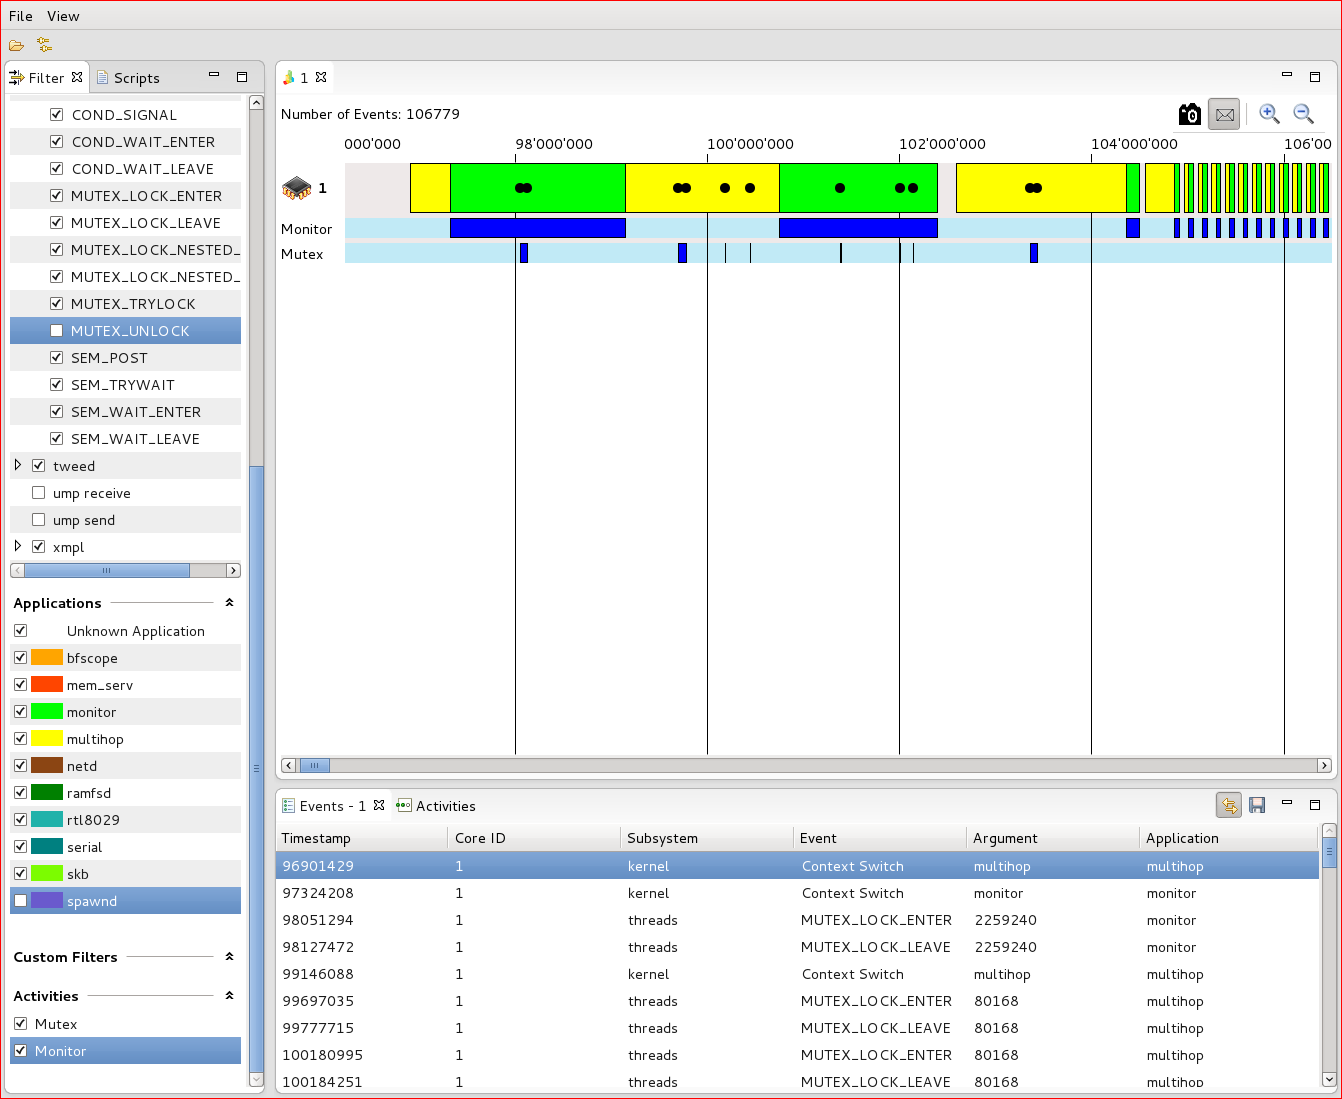
\includegraphics[width=1\textwidth]{images/aquarium-filters.png}
	\caption{Screenshot of Aquarium where core 0 is filtered out, as well as
	certain events and applications.}
	\label{fig:aquarium-filters}
\end{figure}

\chapter{Performance Analysis}

\section{Introduction}

This chapter analyzes the performance of the tracing framework only inside of
Barrelfish. The analysis tool Aquarium is not analyzed for its performance, as
it is intended to run \emph{``offline''} in the sense that if it is fast enough
the consume the data on live mode from a Barrelfish machine, it is considered to
be fast enough. The impact on performance is also a lot bigger on the tracing
inside of Barrelfish; This stems from the fact that if you do not want to
analyze trace data, you simply do not start Aquarium, and if you want to analyze
data, you are willing to wait until the analysis is performed. Looking at the
tracing framework in Barrelfish, it is on one hand less easy to disable -- once
compiled into the system, a certain overhead will exist -- and on the other hand
it is important that the tracing does not affect measured code too heavily, or
it will become useless.

\section{Memory Overhead}

The memory overhead for buffers inside the tracing framework is constant during
the entire runtime of Barrelfish, as the only used buffers are allocated at
startup of the system. The used buffer space currently consists of two main
parts that exist for each core:

\begin{description}
	\item[Application Buffer] Up to 128 currently running applications can be
		stored per core.
	\item[Event Buffer] Up to 8000 Events can be stored per core, where
		ringbuffer containing these events is cleared during a flush process.
\end{description}

To store an event or an application 16 bytes are used. As the tracing framework
works independently of the actual number of cores, the number of cores is
bounded assuming a limit of 64 cores. This leads to the following memory usage:

\begin{equation}
	M = (128 + 8000) * 16 \textrm{B} * 64 = 8323072 \approx 8 \textrm{MB}
\end{equation}

In addition to those buffers, a handful of pointers are stored, which in total
use less than 1 KB of memory. Therefore that the total amount of memory that the
tracing framework uses is 8 MB, which does not vary over time.

\section{Execution Time Overhead}

\subsection{Cost to Trace a Single Event}

We benchmarked the number of cycles that it takes to trace a single event in the
tracing framework. We tested both the case where the Subsystem is enabled,
i.e.~we are interested in the event for which the \texttt{trace\_event} function
is called, and the case where we are not interested in the even that is traced,
i.e.~the Subsystem is disabled. The \emph{``enabled''} case is straightforward
to benchmark, but we also think the \emph{``disabled''} case is interesting, as
it might be often the case that code is instrumented with a lot
\texttt{trace\_event} calls, even though you are currently not interesting in
analyzing this part of the code. Since we added the functionality do dynamically
disable the appropriate Subsytems, it is also important to know by what degree
the execution of the code will be slower, compared to removing the statement
from the actual code.

The results of the benchmark can be seen in Figure \ref{fig:boxplot}. The
benchmark shows that on the machine \texttt{nos5}, the average number of cycles
that it takes to trace an event, when the Subsystem is enabled is 40.384. The
average number of cycles for a call, when the Subsystem is disabled is 9.950.

It can be seen that both benchmarks returned very stable results - there are a
few outliers, but the vast majority of the events are closely around the
average. Both benchmarks have been run twice with 1000 measurements each run.

\begin{figure}[htb]
	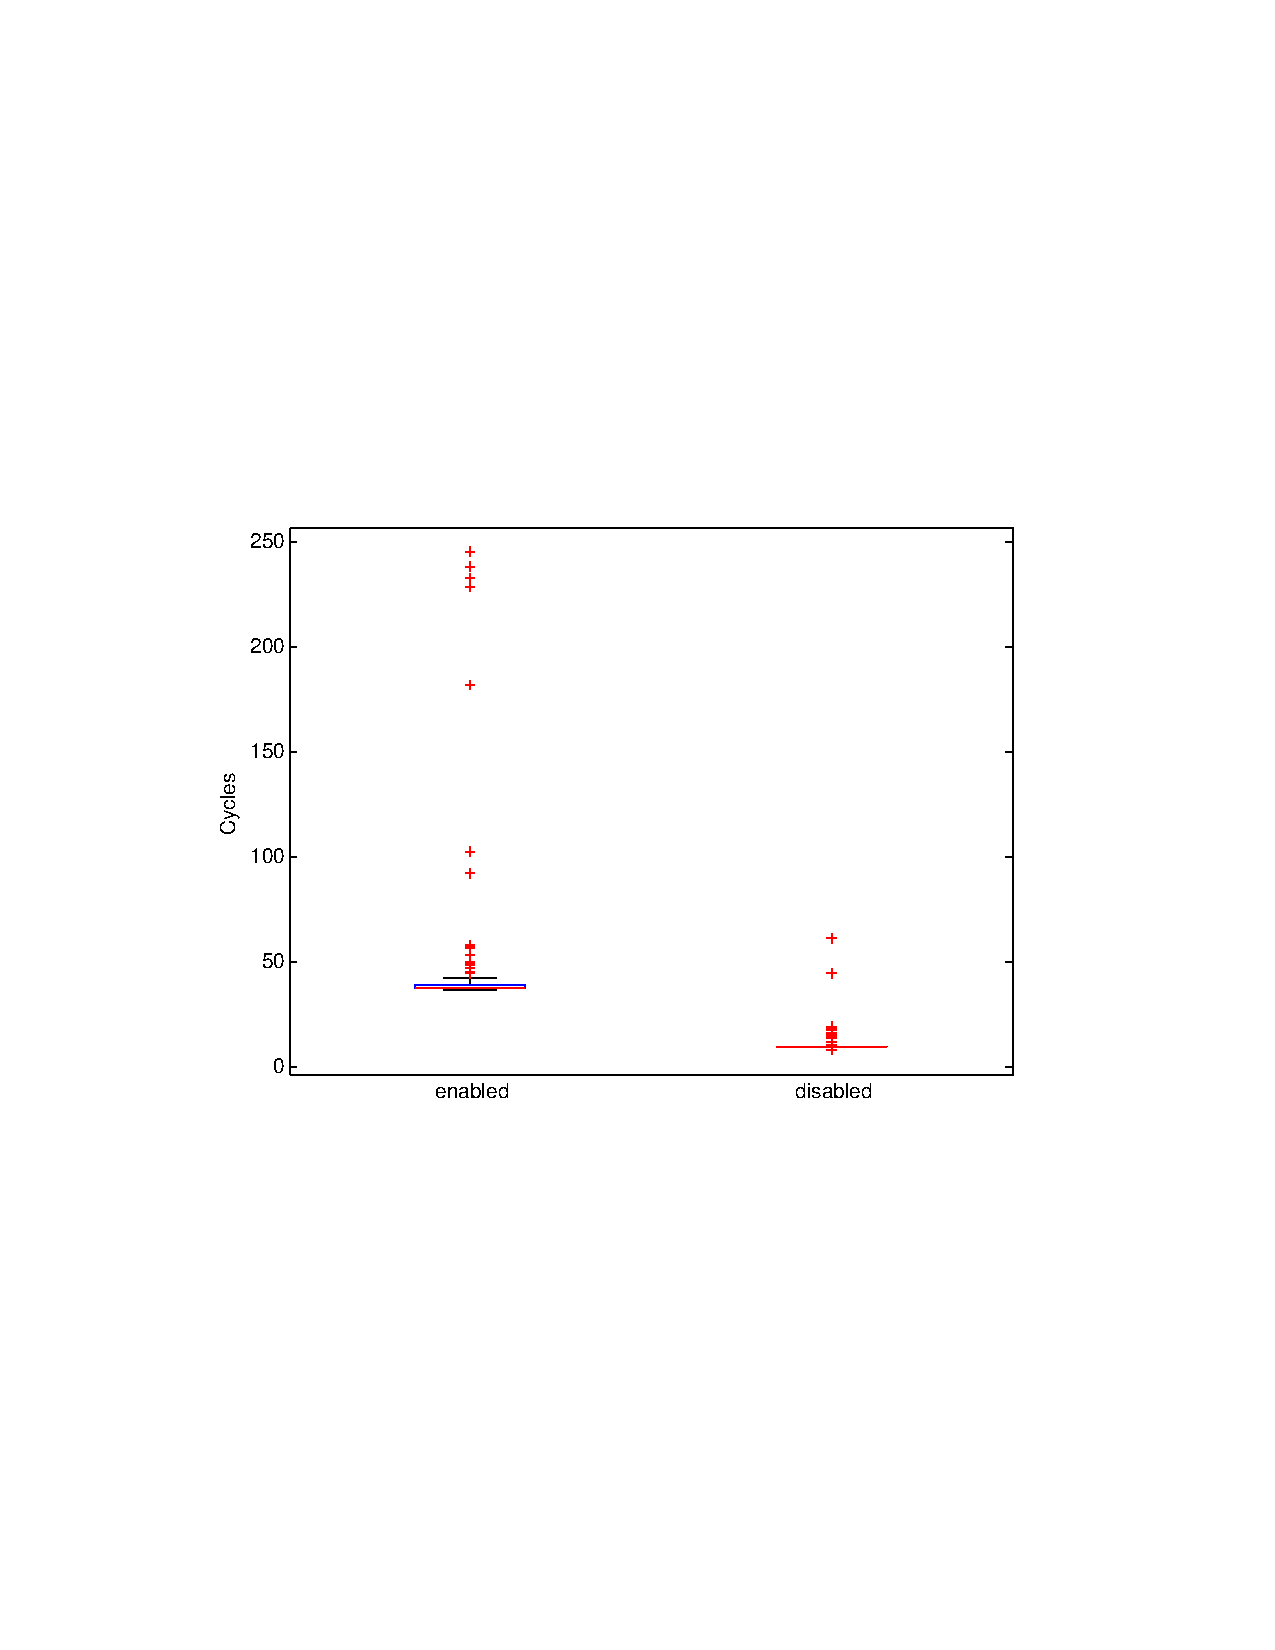
\includegraphics[width=1\textwidth]{images/boxplot.pdf}
	\caption{Boxplots showing the number of cycles that it takes to trace a
	single event. On the left: The Subsystem is enabled, i.e.~the event is
stored in the buffer. On the right: The Subsystem is disabled, i.e.~the event is
not stored in the buffer.}
	\label{fig:boxplot}
\end{figure}

\subsection{Cost to Flush}

The cost to flush the collected trace data can vary a lot depending on the
destination onto which is flushed: Directly on the console, using Bfscope to
send it over the network, etc. As the tracing framework is not intended to be
used in a way where flushing is performed during a measurement, but afterwards,
we did not do measurements for the different flushing methods. We only want to
mention that flushing, especially over the network, is not to be considered a
lightweight operation that can be done at any time during your code, without
potentially affecting the outcome of the tracing heavily.

% vim:set spell spelllang=en_us tw=80:



\end{document}
